%================================================================================================%
% Codex longform document template for LuaLaTeX, provided by T.N. Dionne                         %
% Forked from a template initiated by Prof. D. Sénéchal (2013) and modified by J. Leblanc (2025) %
% This template is offered free of warranty and may be freely modified                           %
%================================================================================================%

%%% Choose between electronic and print versions
\documentclass[titlepage,oneside,letterpaper,11pt]{book} % electronic
%\documentclass[titlepage,twoside,letterpaper,openright,12pt]{book} % print

%%% Insert date here
\def\DATE{\color{red}DATE DU DEPOT FINAL\color{black}}

%------------------Math Setup-------------------

%%% Packages

\usepackage{amsmath}        % math environments
\usepackage{mathtools}      % tools for math formating
\usepackage[nice]{nicefrac} % nicer fractions
\usepackage{cancel}         % allows to scratch expressions.
\usepackage{slashed}        % allows to slash individual characters.
\usepackage{xargs}          % better handling of optional arguments for commands
\usepackage{braket}         % convenient Dirac notation

%%% Custom macros

\usepackage{macros} % custom latex macros (macros.sty)

%------------Fonts (Body and math)--------------

%%% Main font (EB Garamond)

\usepackage{fontspec} % Finer font selection (requires Lua/XeLaTeX)
\setmainfont{EB Garamond}[
  Ligatures   = TeX, % ligatures
  OpticalSize = On, % optical weight adjustment
  % Numbers     = OldStyle, % can be a little hard to read
  SmallCapsFeatures = {LetterSpace=5} % Adds spaces for small caps
]

%%% Math font (Libertinus Math)

\usepackage{unicode-math} % Finer math font selection
\setmathfont{Libertinus Math}[ % Nice neutral universal math font
    Scale=MatchLowercase
]
\setmathfont[ % Adding back a familiar mathcal
    range = {\mathcal, \dagger, \ddagger},
    Scale = MatchLowercase
]{Latin Modern Math}

%-----------------Misc packages-----------------

\usepackage[french]{babel} % language support
\usepackage{setspace} % line spacing
\usepackage{cite} % in text citations
\usepackage{microtype} % small typography tweaks
\usepackage{graphicx}		% figure insertion
\usepackage{subfig}			% allows for subfigures
\usepackage{geometry}		% document geometry
\usepackage{fancybox}		% boxes, frames etc
\usepackage{url}            % typographically sound URLs
\usepackage{float} % Fixes hacky geometry problems
\usepackage[
format    = hang,
margin    = 5mm,
font      = small,
labelfont = bf,
labelsep  = space
]{caption} % tweak caption layout and format
\usepackage{csquotes} % For quotes
\newcommand\itsym{$\bullet$} % symbole pour les listes

%--------------------Tables---------------------

\usepackage{array} % tabular functions
\newcolumntype{C}{>{$\displaystyle}c<{$}} % centered math column
\newcolumntype{L}{>{$\displaystyle}l<{$}} % left aligned math column
\newcolumntype{R}{>{$\displaystyle}r<{$}} % right aligned math column
\renewcommand{\arraystretch}{1.5} % vertical spacing of tables
\usepackage{dcolumn} % allows for aligning of values wrt to the decimal
\addto\captionsfrench{\renewcommand\frenchtablename{{\FBfigtabshape Tableau}}} % rename table name (french)

%---------------General layout------------------

\usepackage{theme/layout}

%-------------Colors and Hyperref---------------

% Pass hyperref options before loading pdfx
\PassOptionsToPackage{
    backref=page,
    pagebackref=true,
    hyperindex=true,
    bookmarks=true,
    pdfa
}{hyperref}

\usepackage[a-2b,mathxmp]{pdfx}[2018/12/22] % ???

% options PDF
\hypersetup{
    colorlinks=true,         % colorise les liens
    breaklinks=true,         % permet le retour la ligne dans les liens trop longs
    urlcolor=URLColor,       % couleur des hyperliens (doit inclure x11names dans xcolor ci-dessus)
    linkcolor=LinkColor,     % couleur des liens internes
    citecolor=CiteColor,     % couleur des liens de citation
    bookmarksopen=true,      % ouvre les signets PDF au départ
}

%%% Choose color theme

\usepackage{colorthemes/colors_marine} % choose a style

%%% Colored boxes

\usepackage{empheq}
\setlength{\fboxrule}{1pt} % sets the border width globally (or locally in a group)
\setlength{\fboxsep}{4pt}  % sets padding between frame and content

% \usepackage{tcolorbox}
% \tcbuselibrary{theorems}
% \tcbset{%
%     highlight math style={
%         colframe=MainColor, % MainColor defined in colorthemes
%         colback=white,
%         arc=4pt,
%         boxrule=1pt,
%         sharp corners
%     }
% }

% % Use a colored box for 'cboxed'

% \newcommand{\cboxed}[1]{\tcbhighmath{#1}}


%-------------------------------------------------------------------------------
% Figures TiKz !!!TODO FIX THIS!!!
\usepackage{tikz}
\usetikzlibrary{
	calc,
	patterns,
	positioning,
    external,
    shapes,
    fit,
    backgrounds,
    arrows.meta,
	positioning,
    decorations,
    decorations.pathmorphing,
    decorations.markings,
    shapes.geometric,
    arrows
}
\tikzexternalize[prefix=figures/pdf/]

\usepackage{pgfplots}
\pgfplotsset{compat=1.16}
\pgfdeclarelayer{background}
\pgfdeclarelayer{foreground}
\pgfsetlayers{background,main,foreground}

\usepackage{theme/tikzstyles}
%%%%%%%%%%%%%%%%%%%%%%%%%%%%%%%%%%%%%%%%%%%%%%%%%%%%%%%%%%%%%%%%%%%%%%%%%%%%%%%%


\begin{document}

%-------------------------------------------------------------------------------
% page titre

\thispagestyle{empty}
\vglue 2cm
\begin{center}
\doublespacing
{
%\sffamily % commenter cette ligne pour un lettrage en roman, avec sérif
{Le modèle de Hubbard} % titre
\\[2cm plus 5mm]
par
\\[2cm plus 5mm]
{\large John Hubbard}
\\[2cm plus 5mm]
Mémoire présenté au département de physique\\
en vue de l'obtention du grade de maître ès sciences (M.Sc.)
%en vue de l'obtention du grade de docteur ès sciences (Ph.D.)
\vfill
FACULTÉ des SCIENCES\\
UNIVERSITÉ de SHERBROOKE\\[1cm plus 5mm]
Sherbrooke, Québec, Canada, \DATE
}
\end{center}
\frontmatter
%-------------------------------------------------------------------------------
% page de composition du jury
% modifier/commenter au besoin

% \newpage
% \thispagestyle{empty}
% \begin{center}
% \vglue 1cm
% Le \DATE \\[1cm]
% {\it le jury a accepté le mémoire de Monsieur Hubbard dans sa version finale.}\\[1cm]
% Membres du jury\\[1cm]

% Professeur Dirac\\
% Directeur de recherche\\
% Département de physique\\[8mm plus 5mm]

% Professeur Plank\\
% Membre interne\\
% Département de physique\\[8mm plus 5mm]

% Professeur Pauli\\
% Président rapporteur\\
% Département de physique\\[8mm plus 5mm]


% \end{center}


%-------------------------------------------------------------------------------
% Page de dédicace

\newpage
\vglue 5cm
\begin{flushright}
À mon idole, GTools.
\end{flushright}


%-------------------------------------------------------------------------------
% Sommaire
\newpage
\onehalfspacing
\addcontentsline{toc}{chapter}{Sommaire}\chapter*{Sommaire}
En gros mon travail est sick est esti.

%-------------------------------------------------------------------------------
% remerciements

\chapter{Remerciements}

\markboth{Remerciements}{Remerciements}
Merci à mon homeboy GTools pour être le motherfucker le plus slick que j'ai jamais connu.

%-------------------------------------------------------------------------------
% tables des matières, des tableaux et des figures, etc.

{
\setlength{\parskip}{0ex}
\tableofcontents
\listoftables
\listoffigures
}

% TODO EXPAND ON THIS, VERY CRISPY
% facultatif: liste des notations (abbréviations) utilisées
% \addcontentsline{toc}{chapter}{Notations}\chapter*{Notations}
% \markboth{Notations}{}
% \input{notation.tex}

%-------------------------------------------------------------------------------
% publications

\chapter{Publications}
\markboth{Publications}{Publications}
Les travaux réalisés au cours de ma maîtrise ont mené aux publications suivantes:
\begin{itemize}
    \item Plein de publications
\end{itemize}

%-------------------------------------------------------------------------------
% corps du document
\mainmatter

% facultatif: introduction non numérotée
\addcontentsline{toc}{chapter}{Introduction} % Add in the intro to the TOC
\chapter*{Introduction}
\markboth{Introduction}{Introduction}
\section*{Titre significatif}

\textit{Une introduction très introductive.}

% \part{Une partie}
\chapter{Éléments de théorie et modèle}


    On travaille dans les unitées telles que $e=\hbar=k_\mathrm{B}=1$.

    \section{Modèle de Hubbard}\label{sec:modele_hubbard}
        \red{MISE EN CONTEXTE}

        \subsection{Hamiltonien}
            

Dans sa forme la plus générale, le hamiltonien du modèle prend la forme suivante dans le contexte de la seconde quantification:
\begin{align}
    \mathrm{H} = \sum_{ij,\sigma} t_{ij}\mathrm{c}_{i\sigma}^\dagger\mathrm{c}_{j\sigma}+U\sum_i\mathrm{n}_{i\uparrow}\mathrm{n}_{i\downarrow}.\label{eq:hamiltonien_hubbard_1_bande}
\end{align}
Les opérateurs $\mathrm c^{(\dagger)}_{i\sigma}$ sont les opérateurs annihilation (création) fermioniques d'un électron sur le site $i$ de spin $\sigma$.
Ces derniers peuvent être exprimés dans la base réciproque via les transformée de Fourier:
\begin{align}
    \begin{split}
        \mathrm{c}^\dag_{i\sigma} = \frac{1}{\sqrt{N}}\sum_\ve{k}\Exp{-i\ve{k}\cdot\ve{r}_i}\mathrm{c}^\dag_{\ve{k}\sigma}
    \end{split}
    \begin{split}
        \mathrm{c}_{i\sigma} = \frac{1}{\sqrt{N}}\sum_\ve{k}\Exp{i\ve{k}\cdot\ve{r}_i}\mathrm{c}_{\ve{k}\sigma}
    \end{split}\label{eq:op_creat_anni_fourier}
\end{align}

\begin{figure}
    \centering
    \scalebox{2.5}{
    % \tikzset{external/force remake}
\tikzsetnextfilename{hubbard_1_band}
\begin{tikzpicture}

    % GRID
    \draw[step=1cm,lightgray,very thin, dashed] (-0.2,-0.2) grid (2.2,2.2);

    \foreach \x in {0,1,2}{
        \foreach \y in {0,1,2}{
            \node[circle,draw=MainColor, fill=SupportColor,inner sep=1pt,minimum size=7pt,] at (\x,\y) {};
        }
    }


    % SPINS
    \begin{pgfonlayer}{foreground}
        \draw[-to, semithick,rotate=90] (-.1,0)--(.1,0) ;

        \draw[-to, semithick,rotate=90] (0.9,-1.06)--(1.1,-1.06) ;
        \draw[-to, semithick,rotate=90] (1.1,-.94)--(0.9,-.94) ;
        \node[right] at (1.05,1.2) {\footnotesize $U$};

        \node[right] at (0,-0.1) {\tiny $j$};
        \node[right] at (1,-0.1) {\tiny $i$};

        \draw[-to, semithick,rotate=90] (1.1,-2)--(0.9,-2) ;

        \draw[-to, semithick,rotate=90] (1.9,-1)--(2.1,-1) ;

        \node[above] at (0.5,0.15) {\footnotesize $t$};
        \draw[-to,black] ($(-.28,0)+(.4,.08)$) arc
        [
            start angle=130,
            end angle=50,
            x radius=0.6cm,
            y radius =0.4cm
        ] ;

    \end{pgfonlayer}

    \end{tikzpicture}
    }
    \caption[Représentation schématique du modèle de Hubbard à une bande.]{Représentation schématique du modèle de Hubbard à une bande. Les cercles sont les sites du réseau et les flèches sont des abstraction des électrons occupant ces même sites. Elles pointent dans la direction du spin de ces électrons. Un bond d'amplitude $t$ entre deux site ainsi qu'un double occupation de coût $U$ sont aussi explicitées.}
    \label{fig:hubbard_1_band}
\end{figure}

\chapter{Méthodes de calcul}\label{chap:metho}
   Tu diagonalise dans le fond.

Ahh et aussi,
\al{
    \int_{a}^{b} f(x)\,\symup{d}x = F(b) - F(a)
}
Et pour un vecteur maintenant:
\al{
\symbf{a}\cdot\symbf{b}\label{eq:dot_product}
}
$\mathcal{R}\mathscr{R}\mathfrak{R}\mathbb{R}\mathbb{C}f$

The quick brown fox jumps over the lazy dog. The quick brown fox jumps over the lazy dog. The quick brown fox jumps over the lazy dog. The quick brown fox jumps over the lazy dog. The quick brown fox jumps over the lazy dog. The quick brown fox jumps over the lazy dog. The quick brown fox jumps over the lazy dog. The quick brown fox jumps over the lazy dog.

The quick brown fox jumps over the lazy dog. The quick brown fox jumps over the lazy dog. The quick brown fox jumps over the lazy dog. The quick brown fox jumps over the lazy dog. The quick brown fox jumps over the lazy dog. The quick brown fox jumps over the lazy dog. The quick brown fox jumps over the lazy dog. The quick brown fox jumps over the lazy dog. The quick brown fox jumps over the lazy dog.

The quick brown fox jumps over the lazy dog.

BTW, this is just the dot product \eqref{eq:dot_product}. This is a woodcock \ref{fig:Estoopi_bird}

\begin{figure}[H]
	\centering
	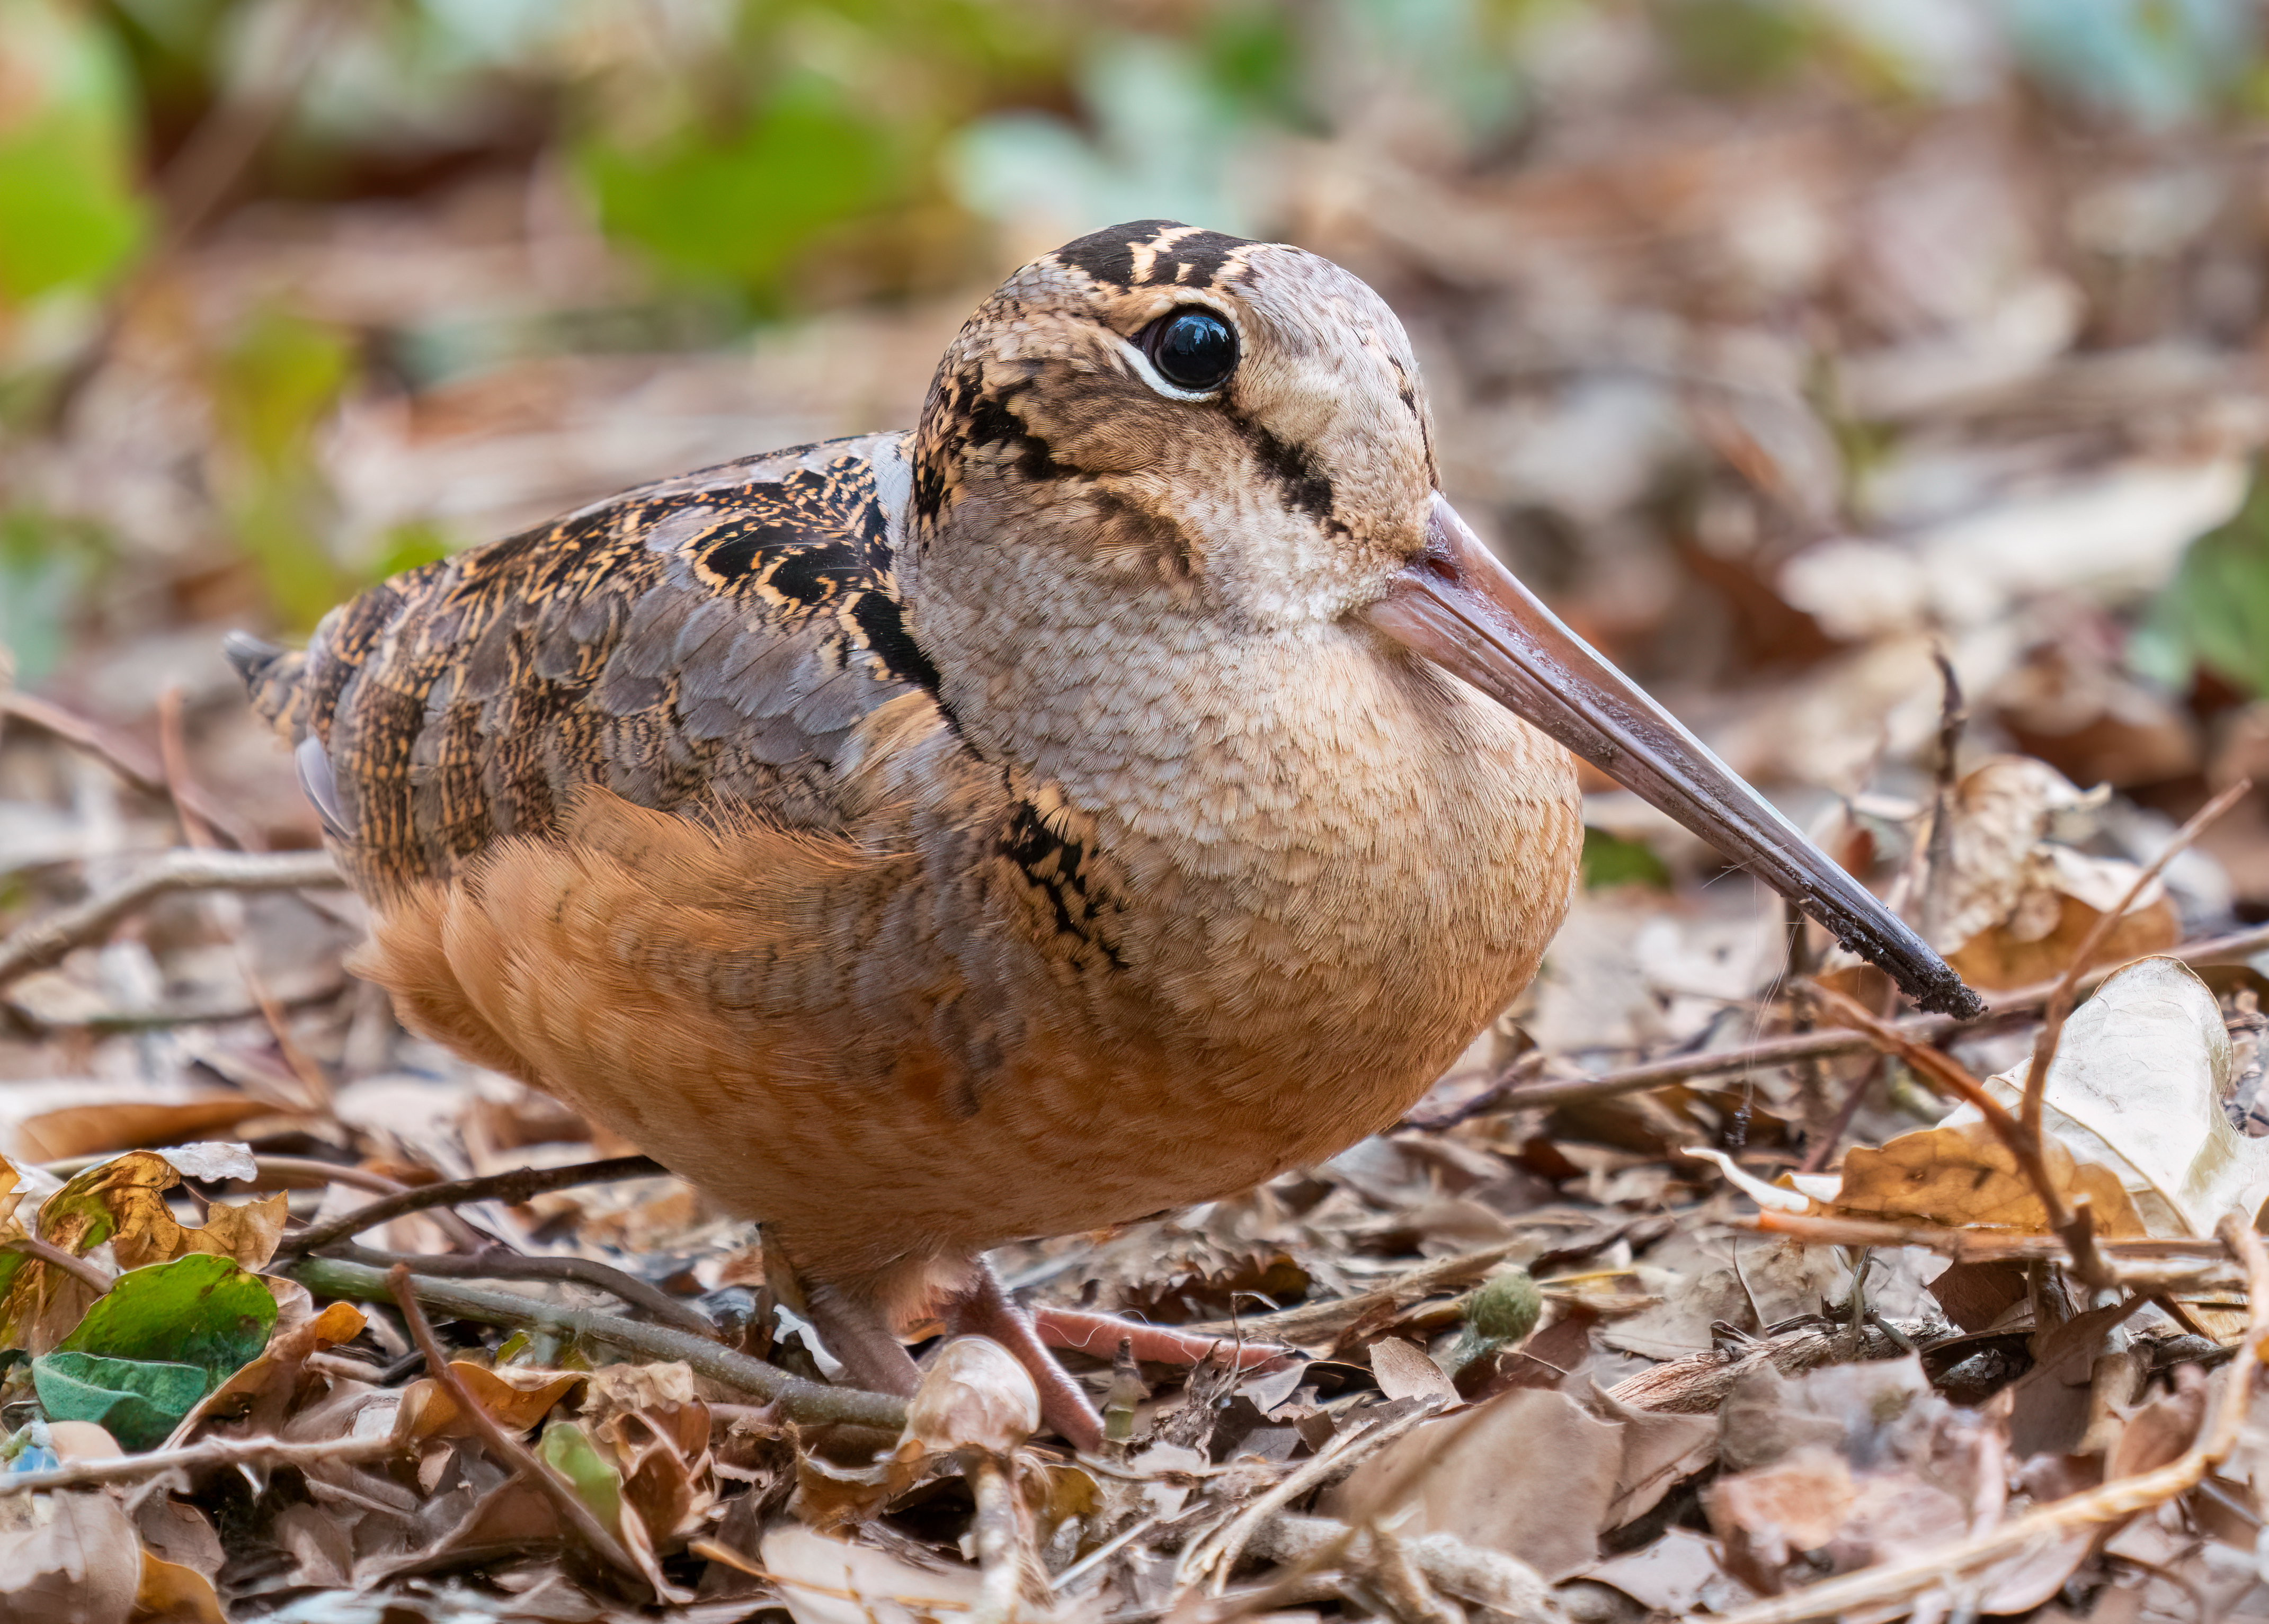
\includegraphics[width=0.5\textwidth]{figures/American_woodcock.jpg}
	\caption{Une bécasse d'Amérique. Un \enquote*{\emph{stoopi-bird}} certifié. En Français, on dit un \enquote{\emph{Oisot}}}
	\label{fig:Estoopi_bird}
\end{figure}

This is nabla $\nabla$. Now this is $\symbf{\nabla}$. How about $\beta$? And now $\symbf{\beta}$... scary!

Now, let $\ve{v}\in\mathbb{R}$

The Wilson loop operator reads as:
\al{
    \boxed{
        \op{W} = \mathcal{T}\Exp{-\oint\D\op{A}}
    }
}
where a creation or annihilation operator would look like $\op{c}_\alpha$ or $\op{c}^\dag_\beta$. Here is just a dagger ($\dagger$) and a double dagger ($\ddagger$). Hence, a general hamiltonian will look like:
\al{
    \op{H} = \sum_{\mu\nu}t_{\mu\nu}\op{c}_\mu^\dagger\op{c}_\nu + \sum_{\alpha\beta\mu\nu}V_{\alpha\beta\mu\nu}\op{c}^\dagger_\alpha\op{c}^\dagger_\beta\op{c}_\mu\op{c}_\nu
}
At equilibrium we say that:
\al{
    \op{\rho} = \Exp{-\beta\p{\op{H} - \mu\op{N}}}
}



%-------------------------------------------------------------------------------
% conclusion

\addcontentsline{toc}{chapter}{Conclusion}\chapter*{Conclusion}
\markboth{Conclusion}{Conclusion}
\input{sections/fin/conclusion}


%-------------------------------------------------------------------------------
% annexes
%\appendix
%\renewcommand\chapterstring{Annexe}
% \appendix
\renewcommand\chapterstring{Annexe}
\chapter{Matériel Supplémentaire}




%-------------------------------------------------------------------------------
% bibliographie

% TODO: SWAP THIS FOR SOMETHING MODERN
%%%%%%%%%%%%%%%%%%%%%%%%%%%%%%%
\singlespacing
\nocite{*} % Shows all references regardless of if cited
\bibliographystyle{CodexStyle/bibstyles/nature-fr} % Use "nature" for english version
\addcontentsline{toc}{chapter}{Bibliographie} % Add bibliography
\bibliography{These}
%%%%%%%%%%%%%%%%%%%%%%%%%%%%%%%

% SO LONG SPACE COWBOY...
% \singlespacing
% \nocite{*}
% \printbibliography

\end{document}
